\subsection{Design Principles}
\label{sec:principle}
\begin{AIbox}
\textbf{Context information density} is the core design constraint for LLM-based agents.
\end{AIbox}

The central challenge in LLM-based agents is not merely context length, but context quality. Recent studies reveal three compounding failure modes that constrain how effectively models can use their input. First, models exhibit strong positional bias when processing long sequences: relevant information placed in the middle of the context is significantly harder to retrieve than information near the beginning or end~\citep{liu2023lostmiddlelanguagemodels}. Second, irrelevant content does not simply go unused; it can actively degrade performance by diverting attention away from decision-critical evidence~\citep{shi2023largelanguagemodelseasily}. Third, the effective context length of LLMs falls far short of their nominal window size, meaning that part of the provided context is functionally invisible during generation~\citep{an2024doeseffectivecontextlength}.

These three phenomena reinforce one another in practice. As context grows longer, positional bias makes middle-positioned evidence harder to retrieve, irrelevant content competes for the model's limited effective attention, and the declining ratio of effective to nominal context length means that an increasing fraction of the prompt is simply wasted. The result is that, beyond a certain point, adding more context does not improve performance and may instead reduce it.

This has direct implications for agent system design. Existing agent frameworks that rely on monolithic prompt assembly often devote a disproportionate share of the effective context budget to scaffolding, control text, and marginally relevant interaction history. Rather than exposing only decision-relevant information, such strategies displace the evidence most needed for the current step, leaving the agent with more context in volume but less context in utility, while still increasing inference cost.

\textbf{From the perspective of context engineering, this problem is best understood in terms of two primary requirements and one secondary representational constraint:}
\begin{itemize}
    \item \textbf{Completeness.} {\small
    All information required for the current decision must be explicitly present in the context, preventing the model from relying on implicit assumptions or hallucinated completions.
    }

    \item \textbf{Conciseness.} {\small
    Irrelevant and redundant information must be eliminated so that attention remains focused on decision-critical signals.
    }

    \item \textbf{Naturalness.} {\small
    The context should remain reasonably natural and semantically legible, especially when aggressive compression or artificial encodings make the representation harder for the model to use. This is an important but secondary constraint: in most agent settings, the dominant failure mode is not lack of natural phrasing itself, but the loss of completeness or conciseness.
    }
\end{itemize}

We argue that completeness and conciseness define the primary design space for context quality in LLM-based agents. Completeness ensures that the model has the information it needs, while conciseness ensures that this information is not diluted by distracting or low-value content. Naturalness still matters, but mainly as a constraint on how information is represented rather than as the main bottleneck in most agent failures. It helps avoid brittle encodings, overly telegraphic summaries, and artificial formats that the model may parse less reliably. Other commonly discussed dimensions can largely be understood within this framework. For instance, recency serves both completeness, because the latest state is often necessary for the current decision, and conciseness, because outdated information is typically no longer relevant. Relevance, rather than being an independent axis, is better understood as a cross-cutting concern: both completeness and conciseness presuppose a judgment of what matters, the former in deciding what must be included and the latter in deciding what should be removed.

\textbf{Critically, the main structural tension is between completeness and conciseness.} This is not merely a consequence of finite context budgets. Even if the context window were unbounded, a structural tension would remain. The tension is structural rather than merely budgetary for at least three reasons:
\begin{itemize}
    \item Including more potentially relevant information improves completeness but weakens conciseness.
    \item Summarization and compression improve conciseness but risk omitting details needed for completeness.
    \item Naturalness can sharpen this trade-off in some cases, because highly compressed or artificial representations may be harder for the model to interpret, but this is typically a secondary effect rather than the dominant constraint.
\end{itemize}

The finite effective context window~\citep{an2024doeseffectivecontextlength} sharpens this tension into a hard practical constraint, but the underlying conflict is structural rather than merely resource-driven. In this sense, context engineering is best viewed not as an equal three-way trilemma, but as a constrained optimization problem centered on balancing completeness and conciseness, with naturalness acting as a supporting constraint on representation.

\textbf{This principle serves as the guiding idea behind the design of GA.} Rather than treating context as a passive byproduct of interaction history, GA systematically optimizes for information density at multiple layers of the system. Its memory hierarchy keeps a lightweight orientation layer visible while leaving richer facts and procedures to explicit reading, preserving conciseness without giving up access to deeper knowledge. Its browser interaction layer represents web pages through semantically structured observations rather than raw HTML, which improves readability while avoiding large amounts of low-value markup in context. Its self-evolution mechanism provides a way to consolidate successful experience into reusable memory and procedures, helping later tasks begin from more compact and task-relevant context. The following subsections describe how each mechanism instantiates this principle in detail.

\subsubsection{Tool Minimality}


GA is built on the premise that general-purpose agency does not require tool proliferation: a small set of well-chosen primitives is sufficient, provided that those primitives are functionally complete for the interactions the agent must perform. Following this premise, \textbf{GA uses only nine atomic tools while retaining broad task coverage} across file operations, code execution, web interaction, and system-level actions. This design is enabled by two supporting properties: \textbf{atomicity}, which constrains each tool to an irreducible primitive capability, and \textbf{compositional generalization}, which allows complex behaviors to be realized through sequences of such primitives. Together, these properties make a small tool set sufficient in practice: the agent does not need a separate interface for each task, only primitives that can be recombined to realize it. Table~\ref{tab:tools} summarizes the complete GA tool set.

Why not simply add more specialized tools? Because tool proliferation introduces system-level costs at two levels:
\begin{itemize}
    \item \textbf{At the prompt level}, each additional tool enlarges the tool schema and associated instructions injected into the context; in multi-turn interaction, this overhead accumulates and occupies effective context budget that should be reserved for task-relevant information.

    \item \textbf{At the policy level}, each additional tool enlarges the action space and increases ambiguity in tool selection. This makes planning more brittle, weakens the stability of tool-use patterns, and increases the likelihood of execution errors and unnecessary retries.
\end{itemize}
Tool minimality is therefore not merely an austerity choice; it is a better operating point that reduces both prompt overhead and decision complexity.

\textbf{Crucially, GA obtains capability through composition rather than tool enumeration.} Its nine tools are designed as reusable primitives, not task-specific interfaces. File workflows emerge from combinations of \texttt{file\_read}, \texttt{file\_patch}, and \texttt{file\_write}; computation and transformation are handled through the general-purpose executor \texttt{code\_run}; and web tasks are realized through the perception--action pair of \texttt{web\_scan} and \texttt{web\_execute\_js}. The remaining tools support the agent's long-horizon control loop: \texttt{ask\_user} acquires missing information, \texttt{update\_working\_checkpoint} maintains short-term task continuity, and \texttt{start\_long\_term\_update} consolidates reusable experience into persistent memory. Thus, GA does not need one tool per task. Broad capability arises from composing a small set of functionally complete primitives. Tool minimality is therefore not a restriction, but the mechanism by which GA preserves general-purpose capability while reducing interaction overhead.

\subsubsection{Hierarchical Memory}
For a general-purpose agent, the main memory challenge lies less in storage itself than in controlling how much information remains in the active context. In monolithic designs, prior interactions, intermediate states, instructions, and execution traces tend to accumulate as the task unfolds. Over long horizons, this causes the default prompt footprint to grow and consume context budget that is also needed for current reasoning and action. GA is designed around this tension: \textbf{rather than treating all retained information as prompt-resident by default, it keeps only a small always-on layer in view and accesses deeper memory only when needed.}

This leads to a layered memory structure in which the always-on layer is intentionally small. GA keeps an L1 memory index in the system prompt as a compact source of orientation: it records where stable resources are located and which global constraints should remain visible, but it does not carry detailed factual or procedural content itself. Richer knowledge is placed deeper in the hierarchy. Stable cross-task facts are kept in a fact layer, while task-specific know-how is stored as SOPs or executable scripts. These resources remain available to the agent through on-demand access rather than through default inclusion in the active context.

Historical interaction data is handled in the same way. Raw sessions are moved out of the always-on layer, archived, and compressed, so that long-run accumulation does not automatically become default prompt growth. This keeps detailed history available without requiring it to occupy the active context during routine reasoning. In this sense, hierarchy in GA is not only an organizational device; it is what keeps the default prompt footprint small while preserving access to richer history and task knowledge when they are relevant.

GA also separates three memory functions that are often conflated in agent systems, and implements them through different mechanisms rather than a single undifferentiated memory store:
\begin{itemize}
    \item \textbf{Working memory} is the task-local continuity buffer. It is updated explicitly through \texttt{update\_working\_checkpoint}, which stores compact task state such as the current objective, constraints, progress, and relevant SOP pointers. This state is then re-injected in subsequent turns together with recent interaction history, allowing the agent to preserve execution continuity across long tasks without reconstructing the full state each time.

    \item \textbf{Always-on memory} is a lightweight orientation layer, not the full persistent memory base. In the implementation, it is injected into the initial system prompt and periodically refreshed during long runs. Its default contents are the working directory, the fixed memory layout, and the compact L1 insight index. This design keeps durable guidance continuously available while avoiding the context cost of loading full L2 factual memory or L3 SOP files by default.

    \item \textbf{Long-term memory} is handled as an explicit post-task consolidation process. Rather than being appended to the prompt at every step, it is written back only when \texttt{start\_long\_term\_update} is triggered after useful experience has been validated. The update procedure follows the memory-management SOP and performs minimal writes to persistent factual memory (L2) or procedural memory (L3), so that only stable and verified knowledge is retained.
\end{itemize}

These layers therefore differ in lifetime, injection rule, update condition, and context footprint.

The resulting benefit is tighter control over the default prompt footprint. As interaction history grows, memory is no longer carried forward by default simply because more turns have occurred. Instead, the always-on layer remains small, while bulkier history and task knowledge stay in deeper storage and enter the active context through on-demand access. This preserves more of the context window for current reasoning and action. Better retrieval focus and stronger persistence follow from the same structure, but they are secondary to this more basic effect: memory does not steadily displace the active-context budget needed for the task at hand.


\subsubsection{Self-Evolution as Experience Consolidation}

If hierarchical memory controls how past information is retained and accessed, self-evolution concerns whether past execution can remain useful beyond the episode in which it occurred.

A general-purpose agent cannot assume that all useful task knowledge is already present in its initial prompt or latent prior. In open environments, many important regularities are local: they concern a specific user's file system, workflow conventions, browser routines, external services, and recurring task patterns. If such knowledge is never retained beyond the current episode, similar tasks may require repeated rediscovery. \textbf{GA is designed to address this problem by supporting experience consolidation across tasks, rather than treating each task as a fully isolated interaction.}

This claim should be stated carefully. Self-evolution in GA is not parameter learning, nor does it imply that every completed task is automatically transformed into persistent knowledge. The underlying model is not updated after each episode. Instead, GA provides a layered external memory structure, explicit update entry points for task-state and long-term memory, and memory-management guidance for deciding what should be retained after execution. In this sense, what can change over time is not the model itself, but the informational environment in which the model operates.

This design is relevant to the context-quality trilemma introduced earlier. Without any mechanism for retaining validated experience, the agent often faces a recurring dilemma on repeated tasks: either replay a longer exploratory process, which weakens conciseness, or act from a shorter but underspecified prompt, which weakens completeness. GA does not eliminate this tension, but it creates a way to reduce it. When useful experience is explicitly consolidated into memory or reusable task procedures, later tasks may begin from a better starting point than pure rediscovery. \textbf{The role of self-evolution in GA is therefore best understood as creating the conditions under which prior successful experience can be reused in a more compact and task-relevant form.}

Just as importantly, GA does not treat all past interaction as equally worth preserving. Raw execution traces contain failed branches, tentative hypotheses, redundant probing, and one-off detours that are useful during search but often undesirable as persistent context. For this reason, self-evolution in GA is better characterized as \textbf{selective consolidation} than as unrestricted memory accumulation. The system provides explicit pathways for updating working state and writing longer-term memory, while its memory-management guidance biases retention toward information grounded in successful execution and away from volatile, weakly verified, or purely situational content. These criteria should be understood as consolidation guidance and operator guidance, not as a claim that the framework already enforces a complete automatic test of validity, stability, or future reuse.

This selective view also clarifies what kind of compression is at stake. GA does not compress all experience into a single canonical representation. Instead, different retained materials occupy different layers of the memory hierarchy. A lightweight insight layer remains visible as a compact orientation signal, while richer factual knowledge, reusable task procedures, and archived session history remain in deeper storage. Self-evolution therefore does not mean that every past task is reduced to one uniform reusable object. Rather, GA provides a concrete path for consolidation through explicit memory-update actions, a layered retention structure, and memory-management guidance, allowing parts of past execution to be preserved in forms that are smaller, more targeted, and potentially more reusable than the original trajectory.

This point also links self-evolution to the two mechanisms discussed above. The relation to tool minimality should be understood carefully. Tool minimality does not by itself produce self-evolution, nor does it establish that fewer tools necessarily yield better consolidation. In GA, however, retained know-how is naturally expressed less as new task-specific interfaces than as reusable ways of sequencing and combining a small set of general primitives. Hierarchical memory, in turn, keeps retained experience from becoming default prompt clutter. In GA, a lightweight orientation layer remains continuously visible, while richer factual and procedural materials are accessed through explicit reading when the agent chooses to inspect them. \textbf{Tool minimality therefore constrains how action is expressed, hierarchical memory governs what remains visible by default, and self-evolution refers to the persistence of selected experience across tasks within that architecture.}

Under this interpretation, self-evolution should be understood not as a guaranteed automatic skill-growth pipeline, but as an architectural capacity for cross-task adaptation. GA supplies the memory layers, update interfaces, and consolidation guidance through which successful experience may persist beyond the episode in which it was acquired. When such retained experience is later read and applied effectively, it can reduce repeated exploratory effort and support better adaptation to a user's local environment. The main claim, however, is architectural rather than empirical: \textbf{GA is built to support experience-driven improvement over time through externalized memory and reusable task procedures, even though the extent and consistency of that improvement depend on what is consolidated, what is later read, and how it is applied in subsequent tasks.}

\subsubsection{Context Truncation and Compression}
\label{sec:context_truncation_compression}

GenericAgent does not preserve the full interaction history verbatim in the active prompt. Instead, it maintains a compact working context under an approximate character-length budget and progressively reduces older material when the accumulated prompt becomes too large. This mechanism is implemented at the prompt-construction level and should not be interpreted as precise token-level window control.

The implementation combines three distinct layers of context management. The first is a \emph{turn-summary layer}. At the end of each turn, the framework appends one short summary entry to its internal summary list: it uses the model-provided \texttt{<summary>} field when present, and otherwise falls back to a simple summary derived from the physical action of that turn. In subsequent turns, the working prompt injects only the most recent 20 such entries. Thus, what is retained here is a bounded list of one-line turn summaries rather than the last 20 turns in full.

The second is a \emph{task-state layer}. Through the explicit tool \texttt{update\_working\_checkpoint}, the agent may write compact task-critical notes such as user constraints, current findings, file paths, or next-step guidance into \texttt{key\_info} and related fields. Once written, these fields are automatically injected into later working prompts. The checkpoint is therefore explicitly updated by the agent and then automatically carried forward; it is not a background mechanism that autonomously rewrites task state on every turn.

The third is a \emph{raw-history maintenance layer}. Older messages are compressed by format-aware, length-driven truncation rather than by semantic importance estimation. In particular, older \texttt{<thinking>}, \texttt{<tool\_use>}, and \texttt{<tool\_result>} blocks may be shortened by retaining only abbreviated head-and-tail segments, while stale embedded \texttt{<history>} and \texttt{<key\_info>} regions may be replaced with placeholders such as \texttt{[...]} . Accordingly, this mechanism should be understood as tagged-content shortening under length constraints, not as selective preservation of semantically important reasoning content.

When such compression is still insufficient, the system trims the stored message history further. Once the serialized history exceeds the configured approximate budget, older messages are removed from the front, and trimming continues until the retained history falls back below a lower target threshold rather than merely touching the limit. During this process, the implementation also performs lightweight structural hygiene: the remaining history is realigned to begin at a user message, and an initial user message containing tool-result blocks may be rewritten into plain text to avoid leaving an orphaned tool-result fragment at the start of the retained context. This supports a narrow claim of basic structural validity preservation during trimming, but not a stronger claim of semantic reconstruction of prior history.

Related mechanisms also help limit prompt growth at specific tool boundaries. For example, some tool paths support file-based offloading of bulky outputs, and some returned content is shortened before reinsertion into the prompt. However, these should be treated only as tool-specific support for prompt-budget management, not as a general automatic externalization mechanism for all large intermediate artifacts.

Taken together, these mechanisms show that GenericAgent maintains a compact decision state without replaying the entire prior trajectory inside the active prompt. More specifically, it combines bounded injection of recent turn summaries, explicitly updated short-term task-state fields with automatic reinsertion, and length-driven compression and trimming of older history under an approximate character-length budget. These mechanisms are intended to make limited active context more sustainable during multi-step interaction. By themselves, however, they should be read as implementation-level prompt-budget management rather than as direct proof of long-horizon task success under a fixed small context window.
\begin{figure*}[t]
    \centering
    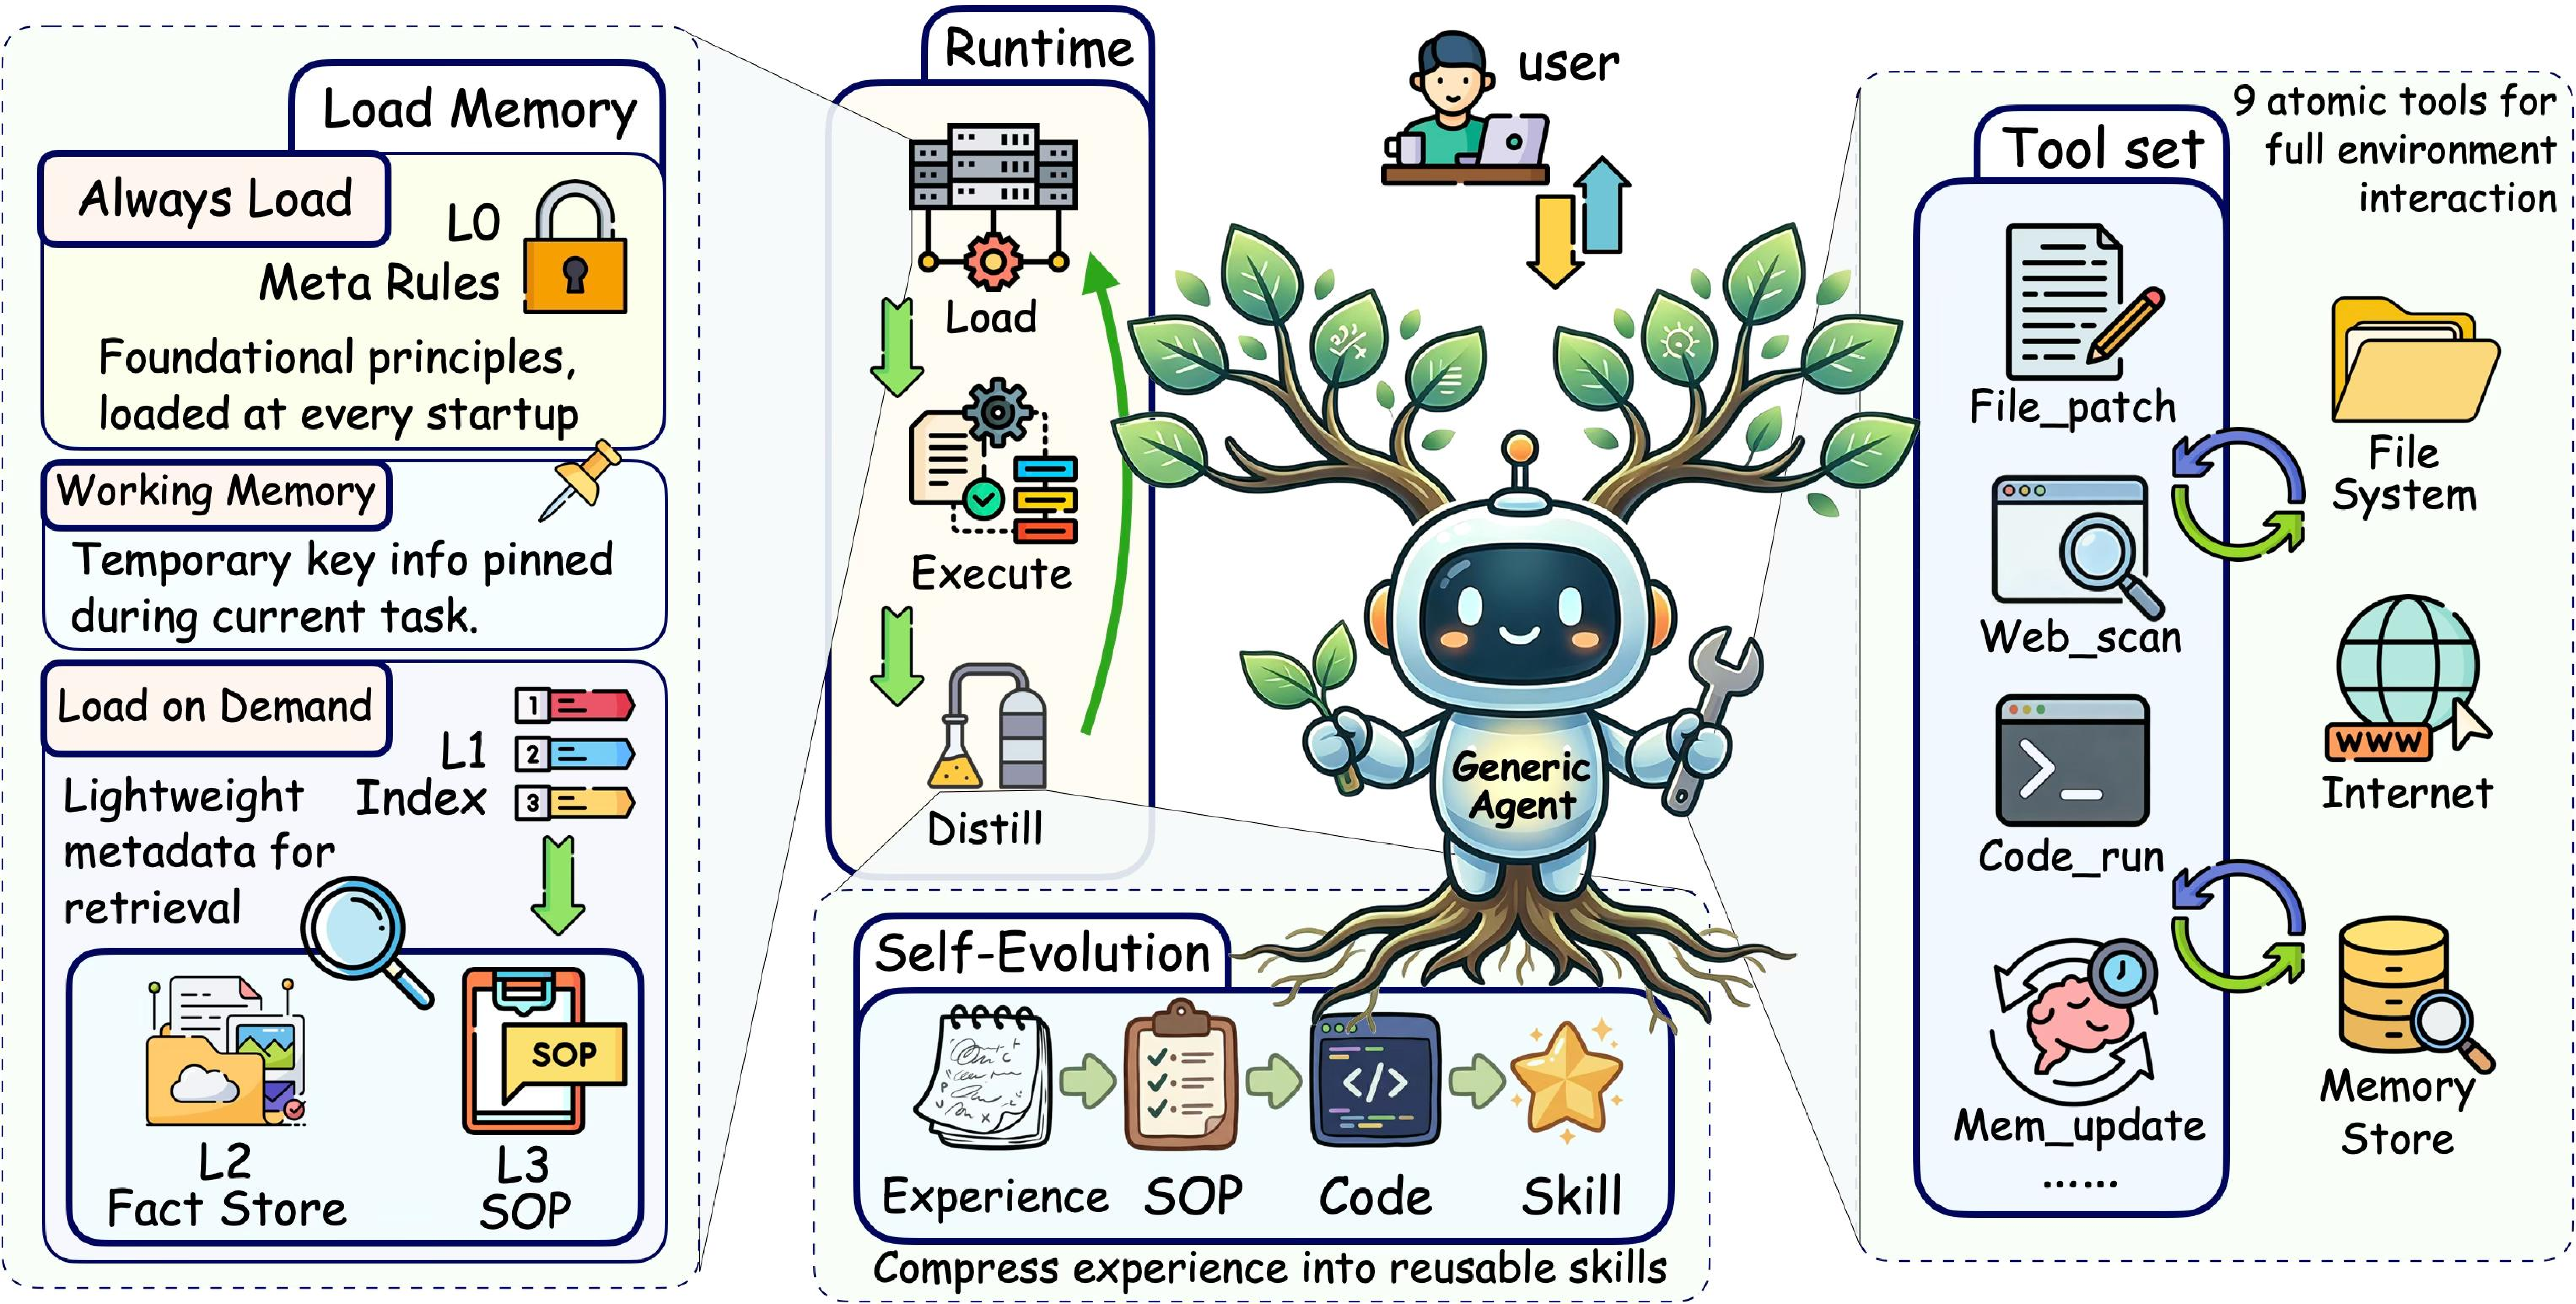
\includegraphics[width=0.98\linewidth]{image/framework_0413.pdf}
    \caption{\textbf{Overall framework of GA.} GA follows a unified agent loop that constructs an execution context from the current task and relevant memory, generates outputs or tool calls, and updates the system through structured feedback.
It is built on four core mechanisms: a minimal tool set, hierarchical memory, reflection-driven self-evolution, and structured browser extraction.}
    \label{fig:agent_loop}
    \end{figure*}
\subsection{Overview of GenericAgent}
\label{sec:overview}
GA is a general-purpose LLM agent system that provides automation over a local computing environment. It enables a compatible LLM backend to operate across browsers, terminals, file systems, keyboard and mouse inputs, screen-based perception, and mobile devices through configurable tool adapters. The system is model-agnostic, allowing the underlying reasoning engine (e.g., Claude, GPT, Gemini) to be replaced without affecting execution logic, tool interfaces, or memory architecture. The overall architecture is illustrated in Figure \ref{fig:agent_loop}.

GA is organized around a unified agent loop that connects the model and the environment. At each step, the system combines global memory with the current task specification to form an execution context. The LLM processes this context and produces either direct outputs or tool calls. Tool execution is delegated to external modules, and the results are returned as structured signals that update the system state. This loop defines a continuous interaction between reasoning and environment feedback, enabling tool-grounded iterative execution.

On top of this loop, GA supports two execution modes. \textbf{Interactive execution} handles user-initiated tasks such as code execution, information retrieval, and file operations. \textbf{Reflective execution} runs in the background and is triggered by schedules or system events. It is responsible for monitoring, memory consolidation, and experience distillation. Both modes share the same agent loop and memory system, differing only in initiation and output handling. To support long-horizon operation, GA defines explicit execution bounds that ensure controllability while preserving interruptibility and scope constraints.

After task completion, GA performs memory distillation. Execution traces are compressed into structured long-term representations and stored in shared memory. These representations are reused across both execution modes, allowing accumulated experience to improve future execution through compression and reuse rather than unbounded computation.

\subsection{Core Components of GenericAgent}
\label{sec:core_design}
Building on the principles in Section \ref{sec:principle}, we describe the core components of GA, covering the atomic tool set, hierarchical memory management, self-evolution, and context compact.

\subsubsection{Minimal Atomic Toolset}
\label{sec:tools}

GA exposes nine atomic tools, grouped into five capability classes.  
The \textbf{File Operations} class includes \texttt{file\_read}, \texttt{file\_patch}, and \texttt{file\_write} for read, precise edit, and block write operations.  
The \textbf{Code Execution} class contains \texttt{code\_run}, which runs Python or Bash in a controlled runtime.  
The \textbf{Web Interaction} class includes \texttt{web\_scan} and \texttt{web\_execute\_js} for low-cost page inspection and precise browser actions.  
The \textbf{Memory Management} class includes \texttt{update\_working\_checkpoint} and \texttt{start\_long\_term\_update} for short-term context maintenance and long-term memory distillation.  
The \textbf{Human-in-the-loop} class is \texttt{ask\_user}, used when user decisions are required. 
Each tool maintains a single responsibility.
These tools form a complete loop covering state observation, action execution, context preservation, and intervention requests.

GA adopts an authority–responsibility aligned permission model.
Authority is strictly defined by the injected toolset, and GA cannot self-escalate beyond it, though \texttt{code\_run} serves as a controlled escalation point by design.
With read-only tools, GA can inspect and reason, but cannot modify any state;
With patch tools, GA can edit text, subject to strict matching and parameter constraints.
With execution and web-control tools, GA can trigger real system actions, while all interactions return structured outputs through the dispatcher, ensuring full traceability.
The objective is not to grant unlimited capability, but to enforce controlled capability with aligned risk and clear accountability.

In terms of tool definition, GA represents tool capabilities as a verifiable schema contract and routes execution through a unified dispatcher.
Each tool defines a name, a description, and a set of parameters described by JSON Schema, all under a consistent type function format.
At runtime, this schema is injected into the interface, allowing GA to produce structured \texttt{tool\_use} calls with explicit names and arguments.
The dispatcher maps each call to a local executor and manages pre- and post-execution handling together with the returned results.
This brings a clear separation between declaration, invocation, and execution. 
GA does not need to know how tools are implemented; it only needs to follow a stable interface contract.
GA then resolves each call against that contract and dispatches it to the concrete handler, separating call semantics from implementation details.

GA implements a \texttt{no\_tool} fallback that auto-triggers when the model produces no tool call, detecting empty responses, truncated output, or unsubmitted code blocks and injecting corrective prompts to re-enter the structured loop.
Turn-based escalation policies further bound autonomous execution: periodic warnings enforce strategy switches, and a hard ceiling forces \texttt{ask\_user}, preventing unbounded runs.


GA also specifically optimizes each atomic tool for decision efficiency and token economy.  
For example, \texttt{file\_read} supports segmented reads (\texttt{start}/\texttt{count}), keyword anchoring, and line-number output, so GA can inspect only relevant regions.  
\texttt{file\_patch} enforces unique \texttt{old\_content} matching and fails fast on zero or multiple matches, reducing silent multi-location edits.  
\texttt{web\_scan} injects a layout analysis algorithm that clones the live DOM, computes per-element visibility, classifies regions as main or non-essential through overlay and partition analysis, and removes covered or hidden elements before serialization, reducing token cost by an order of magnitude compared to raw DOM output.
\texttt{web\_execute\_js} returns action results plus page-change observations, so many workflows proceed without another full scan.  
GA does not merely expose raw operations.  
It recasts real-world operations into low-ambiguity, verifiable, and cost-aware decision interfaces. 
\texttt{code\_run} is restricted to one invocation per turn, ensuring each result is observed before the next action is planned.

In summary, GA is not designed to make the model "do more."  
It is designed to define what can be done, constrain how it is done, and record what was done.  
Through atomic tool abstraction, schema contracts, unified dispatch, and structured receipts, GA aligns capability boundaries, risk boundaries, and accountability boundaries within a single operating framework.

\subsubsection{Hierarchical Memory Architecture}

GA’s memory management is implemented as a layered retrieval-and-update workflow rather than full-history appending. It organizes knowledge through hierarchical structuring, on-demand retrieval, and procedural consolidation.
This design helps the agent stay coherent in long runs and turn validated experience into durable knowledge.

GA starts with a global meta-memory layer.  
This layer defines the memory map, core rules, and update boundaries.  
At task start, GA injects a global memory scaffold as the initial frame.  
The full meta-SOP content is loaded on demand via file reads rather than always preloaded.
It gives the model a shared frame of reference before execution.  
The model knows how memory is organized, what each layer is for, and how updates should be handled.  
This reduces arbitrary writes, historical misreads, and cross-task leakage.

Below the meta-memory, long-term memory is split into four layers with distinct roles.
\textbf{(1)L1 is the index layer.} 
It stores compact pointers, including high-frequency entry points, keyword mappings, and a small set of hard constraints.  
Its main role is fast navigation. It enables efficient memory routing and ensures that relevant information can be quickly located. It works as a directory that guides GA toward appropriate SOPs, factual records, and core constraints for a given task type.
\textbf{(2) L2 is the fact layer.}
This layer stores verified and stable factual information that remains valid over long periods.
Admission is strict.
It includes environment paths, fixed configurations, persistent constraints, and system properties that can be repeatedly confirmed.
Information is only written into L2 after it has been validated through execution and proven reusable across tasks.
Transient states, one-time events, and unverified hypotheses are excluded.
Updates to L2 are performed through small and traceable modifications rather than large-scale overwrites.
This design prevents short-term noise from being stored as long-term facts.
\textbf{(3) L3 is the SOP layer.}
This layer stores reusable procedural knowledge.
It includes task workflows, preconditions, key execution steps, common failure cases, and corresponding debugging or recovery strategies.
Entries are expected to come from action-verified execution and to show reusability across tasks.
Only knowledge that can directly guide error analysis or be reused in future tasks is included in this layer.
\textbf{(4) L4 is the raw session archive layer.}  Unlike L1-L3, L4 is not designed for frequent direct injection into the runtime context.
Its role is persistence and traceability. It stores historical execution sessions so the agent can reconstruct prior trajectories, audit past decisions, and recover task context when needed.
In other words, L4 acts as the long-horizon evidence base, while L1-L3 remain the operational memory layers for routing, factual constraints, and reusable procedures.

Conceptually, GA follows an L1→L2/L3 routing chain. L1 for localization, then selective retrieval from L2/L3 when needed. In practice, this is enforced by tool calls and prompt policy, not a hardcoded mandatory pipeline.
This layered workflow improves both retrieval efficiency and execution reliability in long-horizon tasks.

During runtime, it uses an on-demand loading strategy. 
GA first injects only the minimal required information, including the meta-memory and the L1 index layer.
Additional factual or procedural knowledge is retrieved only when needed during execution.
This reduces irrelevant context noise and improves token efficiency.
It also ensures that context budget is allocated to task-relevant information.

For long-term consolidation, GA uses a triggered commit mechanism instead of immediate writing.
When information is identified as potentially valuable, it enters a validation stage.
Its usefulness and reusability are checked before being committed.
Only verified information is intended to be written into L2 or L3 through small, incremental updates.
The L1 index is updated accordingly. This separation between execution and memory writing reduces incorrect updates and prevents memory bloat.

In addition to long-term memory, GA maintains a session-level working memory.
It is treated as short-term operational cache and is not automatically promoted to long-term memory unless it satisfies the consolidation criteria.
It mainly records the current goal, intermediate conclusions, key constraints, and next actions.
This memory is continuously injected across turns to maintain task continuity.
After each step, a compact summary is generated to form a rolling execution trace.
This prevents degradation of context quality in long conversations.


\subsubsection{Self-Evolution Capability in GA}
\label{sec:self-evolution}
GA implements self-evolution as an explicit operational loop: at each cycle, the agent retrieves prior experience, selects a strategy under current constraints, executes actions through external tools, and feeds grounded observations back into the next step. Capability growth is therefore not an implicit side effect of reasoning, but a visible process in which each iteration can be inspected, corrected, and improved.

A key enabler of this loop is \textbf{the strict separation between atomic tools and evolving task capability.} The tool layer remains stable and task-agnostic, covering only fundamental operations such as environment access and execution, while task-specific strategy is represented in reusable skills and SOP-like knowledge units. Because strategy is externalized from tool implementations, GA can evolve by updating reusable procedures and decision patterns without modifying the base toolset, which reduces regression risk and keeps the system maintainable.

\textbf{Hierarchical Memory makes long-horizon self-evolution stable.} At task startup, GA injects a compact capability index into the system prompt, from which the agent can selectively load detailed procedures on demand; during execution, it records compact step checkpoints that preserve key decisions, progress, and immediate intent. By storing concise continuity signals instead of full history at every turn, GA avoids repeated re-derivation of context and reduces strategy drift in long tasks.

\textbf{Reliable self-evolution depends on controlled consolidation rather than raw trace accumulation.} GA updates long-term memory only at designated consolidation points, such as subgoal completion or failure-recovery transitions, and distills trajectories into transferable knowledge. Successful strategies, reusable decision criteria, environment constraints, and failure anti-patterns are retained, while transient logs and unstable branches are filtered out to prevent memory pollution.

\textbf{Failure correction as an evolutionary safeguard.} 
Reliable self-evolution requires that repeated failure triggers policy correction rather than blind repetition. GA escalates from error-aware retry to environment probing and then to strategy replacement or external intervention under uncertainty or irreversible risk. This ensures that repeated failure triggers policy correction instead of blind repetition, so the evolution process remains directional and reliable over time.

\section{Emergent Capabilities from a Minimal Architecture}
When an agent is constrained to a minimal executable core and exposed as a standard command-line program, several mechanisms often treated as “advanced framework features” emerge naturally at low cost. In GA, two representative emergent capabilities are: (1) subagent through recursive self-invocation, and (2) watchdog behavior through polling and conditional checks.

Many agent systems implement subagents and event handling as separate architectural modules. 
In GA, these are not predefined subsystems.  
They arise from a small set of stable primitives. These primitives include a callable agent entry point, a unified tool interface, a lightweight interaction protocol, and periodic condition checks.

\textbf{Self-Hosted CLI as the Primary Interface.}
This is realized through a self-hosted CLI model. In GA, the command line is not a wrapper around an internal platform; it is the native execution surface of the system. Tasks can be launched with arguments or kept running in the background. Inter-process coordination uses a simple file-based protocol: inputs are written to a task directory, outputs are persisted to disk, and external processes can append instructions or intervene at any time. GA therefore does not require plugin frameworks, event buses, or dedicated orchestration layers to support higher-level behavior. 

\textbf{Subagent as Recursive Self-Invocation.}
Once the agent can be invoked programmatically via CLI, subagents follow naturally. 
A parent agent launches multiple identical instances to handle subtasks.
A subagent is not a special object. It does not require a dedicated manager. 
Parent and child are simply independent processes that follow the same interaction protocol.
This design brings two advantages. 
First, context is naturally isolated. Each instance maintains its own history. 
Subtasks do not interfere with each other. 
Second, the implementation is simple. Parallel execution, progress tracking, instruction updates, and intervention all reuse existing primitives. No extra communication layer is required.

\textbf{Watchdog as Polling-Based Triggering.}
Similarly, once the agent can be invoked programmatically, a watchdog can be implemented through an external loop. 
GA periodically checks conditions and triggers tasks when needed. 
The mechanism is simple: polling, condition mapping, and task injection.
There is no need for an event bus. 
The trigger only decides whether a new task should be created. 
Execution still follows the standard task pipeline. 
This keeps triggering logic decoupled from execution. 
Rules can be maintained as standalone scripts. They can evolve without changing the core runtime.

\subsubsection{Context Truncation and Compression}
\label{sec:context-truncation}

GenericAgent operates within a finite context window and must keep the
cumulative conversation size below this limit without access to a precise
tokenizer or LLM-based summarisation.  Instead, all budget accounting uses
a character-domain heuristic:

\begin{equation}
  C_{\mathcal{H}} = \sum_{m \in \mathcal{H}} \mathrm{len}(m),
  \qquad
  B = \alpha \cdot W_{\text{tokens}},
  \quad \alpha \approx 3 \;\text{chars/token},
  \label{eq:char-budget}
\end{equation}

\noindent
where $\mathrm{len}(m)$ denotes the character length of message~$m$
after JSON serialisation, $W_{\text{tokens}}$ is the configured token
window, and $\alpha$ converts the token budget to a character
budget~$B$.  All comparisons stay in the character domain, and no
conversion back to token counts is ever performed.  This heuristic is
slightly conservative for ASCII-dominated content ($\sim$4 actual
chars/token), which causes mildly early eviction---a safe failure mode.
For CJK content the situation reverses: each character typically consumes
1--2 tokens, so the $\alpha{=}3$ ratio underestimates token usage by
3--6$\times$, risking delayed eviction and potential context overflow.

Context is managed by four co-operating mechanisms, ordered from finest
to coarsest granularity.  We also describe an auxiliary schema-elision
optimisation that reduces the tool-definition overhead.

%% ---- Stage 1 ----
\paragraph{Stage 1: Tool-output truncation.}
Each tool handler truncates its return value \emph{before} it enters the
message history, using a symmetric head--tail policy: when the output
exceeds a threshold~$L$, the first and last $L/2$ characters are kept
and the middle is replaced by an ellipsis.  Table~\ref{tab:tool-truncation}
lists the thresholds for outputs that enter the LLM context.

\begin{table}[h]
\centering
\caption{Per-tool truncation thresholds for content entering the LLM context.}
\label{tab:tool-truncation}
\begin{tabular}{lr}
\toprule
Tool / mode & $L$ (chars) \\
\midrule
\texttt{code\_run}                          & 10\,000 \\
\texttt{web\_execute\_js}$^{\dagger}$       &  8\,000 \\
\texttt{web\_scan} (\texttt{text\_only})    & 10\,000 \\
\texttt{web\_scan} (HTML)$^{\ddagger}$      & 35\,000 \\
\texttt{file\_read}                         & ${\sim}$1\,280/line; 20\,000 total \\
\bottomrule
\multicolumn{2}{l}{\footnotesize $^{\dagger}$\,With \texttt{save\_to\_file},
  the full output is written to disk; only a short preview enters the history.} \\
\multicolumn{2}{l}{\footnotesize $^{\ddagger}$\,DOM-level character budget
  (subtree pruning), not head--tail truncation.}
\end{tabular}
\end{table}

%% ---- Stage 2 ----
\paragraph{Stage 2: Tag-level compression.}
Older messages accumulate redundant content inside well-known XML tags
(reasoning traces, tool invocations, working-memory snapshots).  A
compression pass, executed roughly every five turns to amortise cost,
addresses this in two ways:
(i)~superseded working-memory blocks (\texttt{<history>},
\texttt{<key\_info>}) are replaced by a short placeholder, since
only the most recent snapshot is informative; and
(ii)~content inside reasoning and tool tags (\texttt{<thinking>},
\texttt{<tool\_use>}, \texttt{<tool\_result>}) is truncated to an
$\sim$800-character head--tail window.
The most recent messages (default: 10) are exempt from compression.

%% ---- Stage 3 ----
\paragraph{Stage 3: Message eviction.}
When $C_{\mathcal{H}}$ exceeds the character budget~$B$
after a new message is appended, the system first re-runs Stage-2
compression with more aggressive parameters (exempting only the 4~most
recent messages), then evicts messages in FIFO order until
$C_{\mathcal{H}}$ falls below a target of $0.6\,B$ or
only 5~messages remain.  The 60\,\% target deliberately over-trims,
providing headroom for subsequent turns.  After eviction, the new leading
message is sanitised to maintain API protocol consistency (e.g.\ orphaned
tool-result references are converted to plain text).  No summarisation of
evicted content is performed; the only mechanism that preserves earlier
context is the working-memory anchor prompt described next.

%% ---- Stage 4 ----
\paragraph{Stage 4: Working-memory anchor prompt.}
After each tool invocation, an anchor prompt is appended to the next
user message.  It contains: (i)~the 20 most recent one-line turn
summaries (each compressed to roughly one hundred characters),
(ii)~the current turn number, and (iii)~a persistent \texttt{key\_info}
block maintained by the agent via
\texttt{update\_working\_checkpoint}.  Because this block is injected
into every user message, Stage~2 collapses older copies to a
placeholder, ensuring that only the latest instance carries the full
payload.  This mechanism provides the sole form of long-range memory
after message eviction.

%% ---- Auxiliary ----
\paragraph{Auxiliary: tool-schema elision.}
Under the text-protocol path, tool definitions are omitted from the
prompt when the schema is unchanged from the previous turn, replaced
by a brief natural-language reminder.  The full schema is periodically
re-sent---either on a fixed turn interval or when accumulated prompt
length exceeds a safety threshold---to prevent model drift.  This
optimisation does not apply to the native API path, which sends the
complete tool definitions on every call.

\subsubsection{Autonomous Exploration}
\label{sec:autonomous-exploration}

Many skill-acquisition tasks are open-ended and require extended
trial-and-error that cannot be driven interactively.  GenericAgent
addresses this with an \emph{autonomous exploration} subsystem---a
closed loop in which the agent plans its own curriculum, executes
tasks without supervision, and crystallises results into a persistent
skill library.

The loop proceeds in four phases:
\textbf{(1)}~a timer-based trigger injects an exploration prompt when
the user is idle;
\textbf{(2)}~a \emph{curriculum planner} inspects the current skill
inventory and generates a prioritised task list;
\textbf{(3)}~the agent executes the next task using its standard tool
repertoire (web search, code execution, file I/O), bounded by a
30-round interaction cap;
\textbf{(4)}~outcomes are written to a structured report, from which
new tools and usage statistics are registered in the skill tree.
Planning and execution are strictly separated: the planner produces a
task list and immediately yields control; execution resumes in the
next invocation.

When no pending task list exists, the agent enters planning mode.
Task candidates are scored along four dimensions using a weighted
sum:
%
\begin{equation}
  S(t) \;=\; w_b\,B(t) \;+\; w_d\,D(t) \;+\; w_u\,U(t) \;+\; w_i\,I(t)
  \label{eq:task-score}
\end{equation}
%
\noindent where $B$ (\emph{breadth}) rewards filling under-populated
skill categories, $D$ (\emph{depth}) rewards enhancing frequently-used
skills, $U$ (\emph{utility}) captures estimated practical value, and
$I$ (\emph{innovation}) favours novel techniques or domains.  Each
dimension is scored on a 1--10 scale.

Breadth and depth are computed from skill-tree statistics:
%
\begin{equation}
  B(t) = 10 \times \max\left(0,\, 1 - \frac{|S_c|}{\bar{S} + 1}\right)
  \label{eq:breadth}
\end{equation}
%
\begin{equation}
  D(t) = 10 \times \frac{u(t)}{u_{\max} + 1}
  \label{eq:depth}
\end{equation}
%
\noindent where $|S_c|$ is the number of skills in the target
category, $\bar{S}$ is the mean skill count across all categories,
$u(t)$ is the usage count of the target skill, and $u_{\max}$ is the
maximum usage count across all skills.  The breadth formula rewards
filling categories that are below average, while the depth formula
prioritises enhancing frequently-invoked capabilities.  Utility and
innovation are estimated by the LLM on the same 1--10 scale.

The weights are initially set to $(w_b, w_d, w_u, w_i) = (0.3, 0.2,
0.3, 0.2)$, prioritising breadth and utility.  After each batch of
autonomous tasks, a \emph{reflection-based adaptation} mechanism
adjusts these weights based on actual usage outcomes.  For each
completed task~$t$, if its predicted score $S(t) > 8.0$ but actual
usage $u(t) < 3$ within 30~days, the weight of the dominant dimension
in $t$'s score vector is reduced by 10\%.  Conversely, if $S(t) <
5.0$ but $u(t) > 5$, the corresponding weight is increased by 10\%.
Weights are then re-normalised to sum to unity.  This feedback loop
allows the system to discover which dimensions best predict practical
value in the user's workflow without manual tuning.

The resulting task list must span at least four distinct skill
categories, preventing narrow concentration.

Each autonomous task then proceeds through a fixed sequence:
\emph{context loading} (retrieve recent history and pending tasks),
\emph{skill search} (query the skill tree for relevant tools and
identify gaps),
\emph{execution} (research, prototype, and validate within a
sandboxed temporary directory),
\emph{report writing} (a Markdown document with machine-readable
metadata tags for automatic skill-tree updates),
\emph{skill crystallisation} (an atomic operation that archives the
report, updates the skill tree, and increments usage counters), and
\emph{task-list advancement}.
Even failed experiments are documented so that future planning rounds
can avoid repeating the same dead end.  The crystallisation step
accepts skill annotations either as explicit arguments from the
caller or, as a fallback, by parsing the metadata tags embedded in
the report.  All artefacts are confined to a temporary directory;
modifications outside this sandbox are logged in the report for human
review, and access to secrets or core source code is unconditionally
prohibited.

Autonomous exploration can be initiated in two ways.  In
\emph{task mode}, an external orchestrator (e.g.\ a cron job)
submits a one-shot task via a file-system mailbox and polls for
results.  In \emph{reflect mode}, a user-supplied callback is polled
at a fixed interval; when it returns a non-empty string, that string
is injected as a new prompt.  The default trigger fires every six
minutes with a fixed prompt directing the agent to consult its
exploration procedure.

The skill tree itself is a persistent two-level map: \emph{categories}
(e.g.\ \texttt{web\_automation}, \texttt{data\_processing}) contain
named \emph{skills}, each recording its associated tool scripts and a
monotonically increasing usage counter.  The tree is managed through
an API that supports querying, mutation, usage tracking, and the
atomic completion operation described above.  No
constraint-enforcement or confidence-scoring logic exists in the
current API; validation is limited to deduplication checks before
insertion.

A separate lightweight log records three kinds of entries---observed
errors paired with corrections, explicit user preferences, and
verified success patterns---which are injected into the system prompt
to bias future behaviour.  This is a passive mechanism: entries are
appended during task review, and their only effect is inclusion in
the prompt context.

Several limitations merit discussion:
(i)~the 30-round execution cap means complex tasks may span multiple
sessions, with continuity managed only through reports and task-list
annotations;
(ii)~the reflection-based weight adaptation is preliminary and has not
yet accumulated sufficient data to validate its effectiveness across
diverse user workflows;
(iii)~the self-improvement log depends on manual curation, limiting
its current influence on agent behaviour;
(iv)~skill-tree maintenance---merging redundant categories,
deprecating stale tools, extending the category topology---remains
entirely manual.

\subsection{Compositional Capabilities from a Minimal Primitive Set}

A recurring pattern in agent framework design is to introduce dedicated subsystems for each new capability, for example a subagent manager and a scheduler daemon. GA takes a different approach. It defines a small set of runtime primitives and composes higher-level behaviors from them. The result is not that these behaviors emerge accidentally, but that their implementation cost is low enough to be realized through combination rather than through new architectural layers.

\textbf{Primitive Set.}
Three primitives underpin all compositions described below:

\begin{itemize}
  \item \emph{Callable CLI entry point.} The agent is a standard command-line program that accepts a task via arguments or files and runs to completion. It can be started in foreground, in background, or in a polling mode.
  \item \emph{File-based interaction protocol.} Cross-process communication uses a directory convention. An input file delivers a task, an output file streams results with round-completion markers, and a reply file continues a multi-round dialogue. Three additional control files provide runtime intervention: one requests graceful termination, one injects context into working memory, and one appends instructions mid-execution.
  \item \emph{Polling loop with hot-reload.} A polling mode loads an external script that defines a trigger condition and a check interval. The runtime evaluates the condition periodically; when it fires, the returned string is dispatched as a task through the standard pipeline. If the script file is modified on disk, it is re-executed in place without restarting the agent process.
\end{itemize}

From these three primitives, four higher-level capabilities follow.

\textbf{Subagent Dispatch.}
A parent agent instance spawns child instances by invoking the same CLI entry point in background mode. Parent and child are homogeneous processes; there is no privileged subagent runtime object. Context isolation comes for free—each process maintains its own conversation history in its own memory space—whereas typical frameworks require explicit memory-scope management to achieve the same effect.

Communication between parent and child uses the file protocol described above. This is not fire-and-forget: the parent can monitor progress by reading the child's output, continue the dialogue by writing a reply, or intervene at runtime through the control files. A verbose flag causes the child to include raw tool outputs, enabling the parent to audit intermediate results rather than relying solely on the child's summary. The coordination overhead is real—the operational protocol prescribes active progress monitoring and timely intervention—but it is expressed entirely through the shared file convention rather than through a separate management layer.

For embarrassingly parallel workloads, this yields a map-reduce pattern. The parent prepares independent input files, spawns one subagent per file, and merges the outputs after all children complete.

\textbf{Watchdog via Polling.}
The polling primitive directly supports watchdog behavior. A trigger script encodes an arbitrary condition; the polling loop evaluates it at a configured interval. When the condition is met, the returned string enters the standard task pipeline. Triggering and execution are thus decoupled by construction: the script decides \emph{whether} to create work, and the unchanged runtime handles the work.

Because the polling loop detects file-modification timestamps and re-executes the trigger script on change, trigger rules can be updated at runtime without restarting the agent process. Operational adjustments—changing a threshold, adding a new condition—require editing a single script rather than redeploying the system.

\textbf{Scheduled Tasks.}
A cron-like scheduling system is built as a single trigger script of roughly one hundred lines. It polls a directory of JSON task definitions, each specifying a schedule, a repeat policy (daily, weekday, weekly, monthly, or once), and a maximum delay window beyond which stale tasks are skipped. Cooldown detection prevents duplicate firing, and execution reports serve as the persistence layer for last-run tracking. The scheduler requires no additions to the core runtime; it is a user-space script composed from the polling primitive and the file protocol.

\textbf{Autonomous Idle Behavior.}
A second trigger script, consisting of fewer than ten lines, illustrates the minimality of the composition. It defines a thirty-minute polling interval and returns a fixed task prompt at each check. When the user has been inactive for half an hour, the agent autonomously selects and executes a self-improvement task from a maintained backlog. The significance lies not in implementation complexity, which remains trivial, but in showing that sustained autonomous behavior emerges from a simple configuration of existing primitives rather than a distinct runtime mode.

\medskip
\noindent
The common thread across these four capabilities is that none required extending the core loop. Subagent dispatch reuses the CLI entry and file protocol. Watchdog and scheduling reuse the polling loop. Autonomous behavior reuses both. The design bet is that a small, stable primitive set with low composition cost yields a wider range of behaviors than a framework that pre-allocates a dedicated module for each one.